\chapter{Design}
\label{chap:design}
Much is still unknown in the research area of the robot economy. This thesis aims to create more knowledge on this theory by attempting to build a proof-of-concept of such intelligent system, by designing and implementing key components of our robot economy software framework (see fig. \ref{fig:robot-economy-in-software}).

In this section we present the design of our software application MusicDAO. MusicDAO is a mobile music streaming and discovery application, with peer-to-peer payment to artists in the form of donations and subscriptions. It implements a few key components (see table \ref{tab:robot-economy-building-blocks-2}) of our framework for the robot economy presented in fig. \ref{fig:robot-economy-in-software}. MusicDAO is fully decentralized by design. This means there are no intermediaries, third parties or proprietary servers needed. It is a first step towards a fully autonomous and zero-cost music streaming industry. It is non-profit by design, as there is no single leader or company controlling it. All users of the app form a community to share audio tracks and transfer money using mobile devices. Any user can join this community, publish their musical works and receive money from its listeners. All participants cooperate in the network, which makes it self-scaling by design.

The overall design of the system can be seen in fig. \ref{fig:architecture}. This describes the interaction between the different components, libraries and frameworks. The following sections explain the designed features, components and design choices.
\\

\tikzstyle{background rectangle}=[thin,draw=black]
\begin{tikzpicture}[show background rectangle]

\node[align=left, text width=0.87\textwidth, inner sep=1em]{
The main goal of MusicDAO is: Distributing the power in the music industry, from centralized platforms to listeners and artists. Meaning: liberating artists from their dependence on money-grabbing platforms, so that they receive 100\% of the subscription/donation money from their listeners.
};

\node[xshift=1.0ex, yshift=-0.7ex, overlay, fill=white, draw=white, above 
right] at (current bounding box.north west) {
\textit{Main goal of our system}
};
\end{tikzpicture}
\\
\\
We build upon the theory of a Decentralized Autonomous Organization (DAO) (see sec. \ref{sec:dao}). This is a piece of software that lives autonomously but also heavily relies on humans to do certain tasks. A DAO has internal capital: some kind of value that is used internally to pay humans or robots to complete tasks.

\begin{table}[]
\centering
\begin{tabular}{|l|l|l|}
\hline
\textbf{Robot Economy component}                         & \textbf{Focus in MusicDAO} & \textbf{Related work} \\ \hline
Peer-to-peer leaderless and self-scaling infrastructure     & \checkmark  &                                    \\ \hline
Resilient communication                    & \checkmark  &                                    \\ \hline
Democratic user engagement                      &    & \cite{osgood2016future}, \cite{meter2017design}                                   \\ \hline
Trustless content sharing and exploration  & \checkmark &                                     \\ \hline
AI for decision making (robot tasks)       &   & \cite{dey2016machine}                                    \\ \hline
Trustless monetary system                  & \checkmark  &                                    \\ \hline

Continuous code evolution and distribution &   & \cite{jentzsch2016decentralized}, \cite{dupont2017experiments}                                     \\ \hline
\end{tabular}
\caption{The main components to achieve a robot economy in software (repeated from ch. \ref{introduction})}
\label{tab:robot-economy-building-blocks-2}
\end{table}

% SIMPLIFY AND CLARIFY THIS ARCHITECTURE IMAGE
\begin{figure}
    \centering
    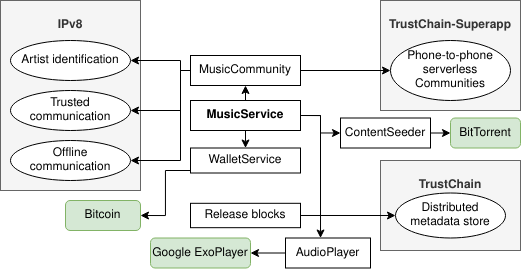
\includegraphics[width=0.6\textwidth]{design/architecture-v2.png}
    \caption{Architecture overview, with in green the external software components. MusicService is the central component in our system}
    \label{fig:architecture}
\end{figure}

% Dit is veel herhaling: verbeter deze sectie (heeft niet veel Body)
\section{Zero-cost autonomous music industry}
We design a system that takes important steps towards a zero-cost autonomous music streaming industry, with no intermediaries. In this utopia, intermediaries that add no real value to the industry receive no money. Artists receive near-100\% of all income as they are the core contributors to the industry. Anyone in the community of artists and listeners can create and share music without contacting a party for a contract or allowance. An open protocol over which money and music is exchanged, can be used with different applications, so that users have a choice of user interface. 

Real-world thriving examples such as Linux or Wikipedia are driven by community and effort instead of profit. Consensus is reached through discussion instead of through pyramid schemes. We envision a similar transition for the digital music industry. The next sections will explain the design of our proof-of-concept of MusicDAO, which aims to be the first piece for reaching a fair music industry. A proof-of-concept of the robot economy will show an important step towards mobile infrastructure for the common good: a system in which participants do not lose money and power to greedy intermediaries. Instead, they will benefit from cooperation. Our framework for the Robot Economy aims for absolute fairness, controlled by the community from the ground up instead of dictated top-down. All funds from users are forwarded directly to the main contributors (in this context, musicians), bypassing all intermediaries.

\section{Zero-server phone-to-phone application}
Traditional Internet services are built around a single server or a set of servers (fig. \ref{fig:centralized-service}). We design a network which only consists of mobile phones (fig. \ref{fig:decentralized-phones}). Every phone cooperates by storing, sharing and validating content. Each mobile phone has access to the same functionalities. The reason for this topology is to prevent monopoly power. In the network, every participant has access to the same functionalities. There is no central server or central database. Its goal is to scale naturally: every participating device contributes resources by hosting content. The computational power and bandwidth capacity grows with the amount of devices requiring these resources.

A key attribute of the network is censorship-resiliency. That means that no single authority (company, institution or government) can remove tracks, or prevent devices from participating in the network. Censorship-resiliency is an important requirement for the system because of the issues described in \ref{sec:problem-description-censoring}. Attempting to build a resilient system while using Internet technologies results in a few key challenges as identified by \cite{pouwelse2012censorship} and \cite{di2014bypassing}. By using a distributed, immutable data structure TrustChain~\citep{otte2017trustchain}, no music data can be censored by any authority. The BitTorrent peer-to-peer file sharing network also prevents censoring and spoofing by using encrypted file transfers and random port selection. As a back-up for internet kill switches, we apply \textit{direct communication} between devices in near range, by using BlueTooth and Wi-Fi direct, as implemented in the TrustChain Superapp decentralized application framework~\citep{mattskala2020}.

\section{Phone-to-phone connectivity}
MusicDAO is designed to have a network consisting of only mobile phones (see fig. \ref{fig:decentralized-phones}). We make this decision for this reason: if it runs well on mobile infrastructure, we can conclude it will run well on better hardware as well. Key challenges to establishing and maintaining such a network are: discovering other devices, network connectivity, longevity and scalability.

\begin{figure}
    \minipage{0.4\textwidth}
        \centering
        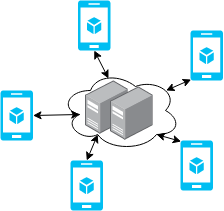
\includegraphics[width=0.6\linewidth]{design/centralized-service.png}
        \caption{Traditional (centralized) Internet service infrastructure}
        \label{fig:centralized-service}
    \endminipage\hfill
    \minipage{0.4\textwidth}
        \centering
        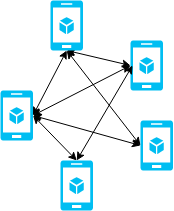
\includegraphics[width=0.6\linewidth]{design/decentralized-phones.png}
        \caption{Peer-to-peer network of phones, as in MusicDAO}
        \label{fig:decentralized-phones}
    \endminipage
\end{figure}

Every device that wants to participate, will try to find other devices to join the network. Every device also keeps track of a routing table, containing public IP addresses of connected and connectable peers, including latency for each peer. This routing table is inspired by the routing table implemented by BitTorrent DHT~\citep{bittorrentbep5dht}. To discover an \textit{initial} list of devices, we use a bootstrap server, which keeps track of other devices on the network to connect with. A bootstrap server should not be necessary when there are devices on the same Local Area Network that can introduce a new device to the network. However, the network of MusicDAO will be sparse at the start. After a few devices are discovered, the bootstrap server can be disregarded, as new devices are then trivially found via neighbor search. 

To support a healthy evolution of the network, every device will maintain a list of connected devices. Devices will send periodic \textit{keepalive} messages to its connected peers to track which are alive and reachable. By doing this, devices can decide which peers are healthy connections. This list should grow to a few dozen, so that there are always connectable peers.

As there will be no central server, each device acts as both a client and server. As devices may be behind routers or other \textit{Network Address Translators} (NATs), establishing a direct connection between devices is not trivial. To achieve this, we use \textit{NAT traversal}. NAT traversal is a set of methods used to establish a connection between devices which have no static, public IP address.

\section{End-to-end music delivery model}
\label{sec:release-model}
In contrary to the current music publishing situation, dominated by IT gatekeeping and oligarchs as visualized in fig. \ref{fig:current-music-publishing-situation}, we present the desired situation in fig. \ref{fig:desired-music-publishing-situation}. This shows the liberation for artists in publishing their content, and the reduction of single-point-of-failure risks. In this system, artists are free in what they upload. In addition, their content can not be taken down by any authority unless there are no participants in the network. The discovery of content is done using open source, transparent systems and listening data is saved and processed locally.

To achieve this situation, a main component of our system is the storage of metadata and audio files for playlists. We design an abstract model for the structure of this metadata, so that the artist is free in the way to release music content. The artist may publish tracks as part of a single, an EP, an album or any other structured list of tracks, as a Release object.

\begin{figure}
    \centering
    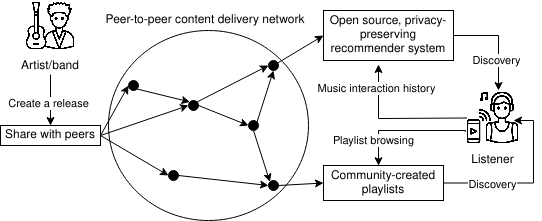
\includegraphics[width=0.8\linewidth]{design/desired-music-publishing-situation-2.png}
    \caption{Desired music publishing flow using a distributed network}
    \label{fig:desired-music-publishing-situation}
\end{figure}

A Release object contains a list of tracks that are published by a clearly identifiable artist or group of artists. It is modeled as shown in fig. \ref{fig:release-model}. Release objects are shared between peers in the network. By discovering many of those objects, a user can see and browse through them to select a track to play. A Release object merely contains metadata of the tracks. We design the network to have a separate channel for downloading the track files. This is to enable fast discovery and searching of Releases, as Release objects have a small byte size. 
\begin{figure}
    \centering
    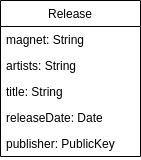
\includegraphics[width=0.2\textwidth]{design/release-model.png}
    \caption{Release blocks structure as seen on TrustChain}
    \label{fig:release-model}
\end{figure}

\section{Identification of participants in permissionless network}
\label{sec:pki-design}
MusicDAO allows any person to participate, and start publishing or listening to music. It requires a permissionless infrastructure, in which artists can be identified. As we design a system that is fully decentralized, we cannot use a central database to record user identities. Therefore every user generates a unique identity to be used in the network, and must be able to give proof of this identity. 

We use a public key infrastructure (PKI) which achieve these goals. Every user stores their private and public key on their device, and only share their public key. The keypair has a mathematical property that allows verification of messages that are signed with a private key. By comparing the public key of a peer with their signed message, anyone can verify the authenticity of the message. MusicDAO will use a PKI to proof ownership of Release objects. All Release objects are signed using the owner's private key and the signature is added to the object. Using these signatures, any user receiving this object can verify its authenticity. We choose to use the public key infrastructure as implemented in the TrustChain-Superapp~\citep{mattskala2020}. This abstracts network identifiers such as IP addresses, which may change over time; so it provides a unique identity per Android phone.

In a permissionless infrastructure, maintaining a record of trustworthy parties is non-trivial. To still establish trust in the legitimacy of artists, we use the TrustChain DLT~\citep{otte2017trustchain}. Using this technology, we record the history of uploaded tracks in an immutable and transparent way. In essence, every artist adds Release blocks to its personal chain, and due to the interlinking mechanism of TrustChain, it is not possible to hide parts of this history. Every participant can view this timestamped history, as it is public by design. This way, an application can inspect the legitimacy of an artist. For example, if an application finds a song X, published by both participant A and B, but the song published by participant A was published later, it can be concluded that A is more trustworthy than B, as B may have copied the song. This is a simple implementation of the Trust on First Use (TOFU) model~\citep{toth2013public}.

This system can also be extended trivially to user ratings, or other interactions between parties, to achieve better measurements of trust. This distributed datastore of immutable and transparent histories then becomes a measure against Sybil attacks~\citep{douceur2002sybil} and artist impersonation.

\section{Peer-to-peer music discovery and sharing}
\label{sec:distributed-storage}
Central to our system is sharing, downloading and storage of audio files and metadata. To design a system which has no middlemen or regulators for publishing Releases( see \ref{sec:release-model}), and has no central control, a distributed storage system is required. This storage system should have the following properties: immutability (data cannot be tampered with), resiliency (data should be available as long as users want it) and rigorous duplication (all objects should be saved on multiple machines). Distributed ledger technology (DLT) allows for these properties, so we design our system with a DLT as a major component.

One implementation of this technology is TrustChain~\citep{otte2017trustchain} which allows for recording transactions between peers in a linearly scaling public ledger. Every peer has its own immutable and public blockchain which shows its history of transactions with others. We choose TrustChain because of its scalability, its trust mechanism, and because it has a native and offline-mode implementation for Android, as described in sec. \ref{sec:sote-trustchain}.

% \section{Peer-to-peer music sharing}  TODO check if this flows well with content above
\subsection{Distributed file hosting}
\label{sec:p2p-music-sharing}
In order to minimize latency for discovering and playing music tracks, while using no central nor high-throughput servers, the network demands participants to upload content continuously. The peer-to-peer file sharing protocol BitTorrent is suitable to share audio files in MusicDAO. We make BitTorrent a design choice as it does not require synchronizing with a global data store, in contrary to IPFS. This means we can build a metadata store independently from BitTorrent. Furthermore, it has a built-in tit-for-tat strategy for file transfers, and it is generally more decentralized than IPFS (see \ref{sec:sote-bittorrent}). BitTorrent also has stable implementations for Android.

We design the app to, by default, seed the content of $\leq k$ Releases, which are sorted in descending order on publication date. This means that the seeding protocol uses a first-in-first-out strategy. This simple heuristic is used because of ease of implementation, because it requires no communication between devices. However, it could lead to unhealthy BitTorrent swarms for music released long ago. A peer-to-peer load balancing mechanism could prevent this but is out of scope for this thesis because of complexity.

Seeding of content should be done as a background process on the phone, so that it is still running when the app is not in use, and therefore maximize the availability of content.  However, this is constrained by networking hardware, data subscription plans and other software running on the phone. The effectiveness of this approach should be evaluated with through experimentation.

\subsection{Distributed search algorithm}
For searching content, we introduce a simple distributed algorithm, based on the more Gnutella search and retrieval protocol~\citep{kronfol2002fasd}. Gnutella is widely used and has over a million users. Pseudocode of our algorithm is shown in alg. \ref{alg:algorithm-distributed-search}. It asks peers around for content tagged with some keyword. When a peer finds a match on their local database, it sends this Release object to the original asking peer. Otherwise it forwards the query to their neighbours, after reducing the time-to-live property by 1. The messages stop being forwarded once their time-to-live property hits below 1. 

\begin{algorithm}
\caption{Distributed algorithm for remote search}
\begin{algorithmic}
\Function{DistributedSearch}{$query, ttl, maxPeers, minResults$}\Comment{Device initiates the search}
    \State $results\gets localSearch(query)$\Comment{Filter local database}
    \If {$|results|\leq minResults$}
        \State $origin \gets myAddress()$\Comment{Address of the device initiating the search}
        \For{$i\gets 1, maxPeers$}
            \State $peer \gets peers[i]$\Comment{Select a random neighbor}
            \State $sendQuery(origin, peer, query, ttl)$
        \EndFor
    \Else
        \State \textbf{return} $results$
    \EndIf
\EndFunction
\Function{OnQuery}{$origin, peer, query, ttl$}\Comment{This is called when a query is received}
    \If $ttl\leq 0$
        \State \textbf{return}
    \EndIf
    \State $ttl \gets ttl-1$
    \State $results\gets localSearch(query)$
    \If {$|results|\le 1$}
      \For{$i\gets 1, maxPeers$}
            \State $peer \gets peers[i]$
            \State $sendQuery(origin, peer, query, ttl)$
        \EndFor
    \Else
        \State $sendResults(origin, results)$\Comment{Send the results back directly to the origin}
    \EndIf
\EndFunction
\end{algorithmic}
\end{algorithm}

\begin{figure}
    \centering
    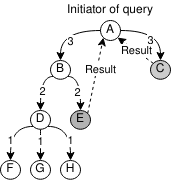
\includegraphics[width=0.3\textwidth]{design/search-algorithm-diagram.png}
    \caption{Search algorithm execution example: node A initiates a search query}
    \label{fig:search-algorithm-diagram}
\end{figure}

Fig. \ref{fig:search-algorithm-diagram} shows a visualization of execution of the algorithm in a small network. Participant A wishes to find a set of results $R$ for query $q$, so it initiates a search query. Firstly it inspects its local database. Because there are $|R|=0$ results, it sends a query to its neighboring peers (B and C). The peers depicted in grey find $|R|\geq 1$ results; they send their result back directly to A and do no other action. Other peers forward $q$ to its neighbors, reducing $q_{ttl}$ by 1. \textit{Time-to-live} hits 1 when arriving in F,G,H so the search terminates. 

\subsection{Content popularity algorithm}
In order to present users with content that is reachable (downloadable), we track \textit{content healthiness}. Content healthiness is the amount of active peers that have and upload some specific piece of content. In the context of music this is the amount of uploaders for a music release (see fig. \ref{fig:release-model}). This idea is heavily influenced by the \textit{swarm health} terminology as part of BitTorrent, which interprets the number of seeders and leechers.

% Explain the algorithm here and extend the section

Our gossip-based algorithm used for spreading information about content healthiness is presented in alg.~\ref{alg:algorithm-content-popularity}. Gossip-based algorithms are suitable in distributed systems because of their simplicity and flexibility~\citep{kermarrec2007gossiping}. Our algorithm is influenced by previous work: the popularity gossiping algorithm present in the Tribler~\citep{pouwelse2008tribler}. 

In essence, the algorithm works as follows: every peer in the network communicates with a few random neighboring peers periodically. The sending peer sends one message to each of its selected peers containing information about how well content (e.g. a musical Release) is available, measured by the amount of devices that have this piece of content. Every peer in the network has a local registration of content popularity, and updates this periodically. All messages are timestamped, so outdated information is removed after time.

\begin{algorithm}
\caption{Gossiping algorithm for content popularity}
\label{alg:algorithm-content-popularity}
\begin{algorithmic}
\State localDatabase $\gets$ Map(key: item, value: health)
\Function{Gossip}{localDatabase, peers, t, margin}
    \Repeat{} Every $t$ ms
    \For{healthItem in localDatabase}
        \If{timestamp $\le$ timestampNow $-$ margin}
            \State localDatabase->remove(healthItem)
        \EndIf
    \EndFor
    \State healthItem$\gets$pickRandom(localDatabase)\Comment{Pick a random item}
    \State orderDesc(localDatabase)\Comment{Order based on health}
    \State healthItem2$\gets$pickFirst(localDatabase)
    \State peer$\gets$pickRandom(peers)
    \State sendGossipMessage(peer, list(healthItem, healthItem2))
    % \If {$|results|\geq minResults$}
    %         \State \textbf{return} $results$
    % \EndIf
    % \State $origin \gets myAddress()$\Comment{Address of the device initiating the search}
    % \For{$i\gets 1, maxPeers$}
    %     \State $peer \gets peers[i]$\Comment{Select a random neighbor}
    %     \State $sendQuery(origin, peer, query, ttl)$
    % \EndFor
    \Until end
\EndFunction
\Function{OnGossipMessage}{items}\Comment{}
    \State localDatabase->overwrite(item)
\EndFunction
\end{algorithmic}
\end{algorithm}

\section{Transparent money flow}
One aim of MusicDAO is to remove predatory intermediaries from the music streaming revenue flow. Figs. \ref{fig:current-money-flow} and \ref{fig:desired-money-flow} visualize the difference of money flow in the current situation and in MusicDAO. It shows that, when intermediaries are cut from the flow, artists will have a higher income for the same fees from the listener. Streaming services and record holders introduce many overhead costs. Our system allows artists to publish their songs without the need to contact a label. The biggest difference in income will be seen for independent artists, as streaming services gives particularly low payouts for unsigned artists.

As we are designing a system with no intermediaries, it should be possible to give money directly to artists. Cryptocurrency allows for peer-to-peer payments which achieve this goal, so we use this in MusicDAO. Cryptocurrency payments will be used for two different functionalities: a user can send a donation to an artist, or a user can pay artists using a monthly subscription system. This subscription system pays artists that the user listened to, using the Artist Income Division Algorithm (see \ref{sec:aida-design}). 

Fig. \ref{fig:desired-money-flow} shows another component: an automated and transparent payment division system. Currently, record holders have the task of paying artists, but the contracts and systems are often opaque and result in slow and low payouts. Automating this process should reduce these problems. We design the transparent payment system to be an immutable record on a distributed ledger, on which a specification of the exact shares per artists are written down.

We choose to use Bitcoin as a cryptocurrency as it has shown to be a fully peer-to-peer, secure and popular payment system, and it does not rely on any third parties to run. It also allows for making a experimentation environment without any high-throughput external servers. 

\begin{figure}
    \minipage{0.6\textwidth}
        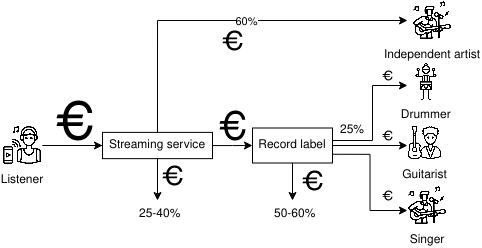
\includegraphics[width=\linewidth]{design/current-money-flow-2.png}
        \caption{Money flow: current situation (simplified)}
        \label{fig:current-money-flow}
    \endminipage\hfill
    \minipage{0.4\textwidth}
        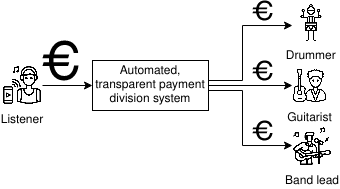
\includegraphics[width=\linewidth]{design/desired-money-flow-2.png}
        \caption{Money flow: desired situation}
        \label{fig:desired-money-flow}
    \endminipage
\end{figure}
Cryptocurrency implementations allow for private/public key-pairs which can be interpreted as a kind of wallet; the funds can only be unlocked by a holder of the private key. In the case of MusicDAO we design the app to include a wallet for every user. To receive money, every artist should share their public key to all of their listeners. To achieve this, the public key of their cryptocurrency wallet is included as a property of the Release objects (see \ref{sec:release-model}).

\subsection{Artist income division algorithm}
\label{sec:aida-design}
To provide a stable income for artists, in the form of reoccurring payments, we design the Artist Income Division Algorithm. This algorithm calculates how subscription money is split into payments to artists. The user can enable a periodic payment. This money is then divided over the artists the user listens to, in proportion to the amount of \textit{interaction} with each artist. 

The algorithm is flexible in the way of measuring interaction. It could be measured in e.g. time listened, plays, feedback in the form of likes or any linear combination of such. These parameters could be voted on by the community. The details of this division is shown in pseudocode, in alg. \ref{alg:aida}. We choose to only create transactions to the first $k$ artists in order to have a constant message complexity for each iteration: $O(k) = O(1)$. This means that artists falling outside of this value of $k$ do not receive money from the corresponding listener, so the value of $k$ becomes a trade-off between network bandwidth usage to process the payments and fairness for artists.

\begin{algorithm}
\caption{Artist Income Division Algorithm (AIDA)}
\label{alg:aida}
\begin{algorithmic}
\State artistInteraction$\gets$Map(key: walletID, value: amount)
\Function{Subscribe}{artistInteraction, fee, k}\Comment{User registers for subscription}
    \Comment{Artist interaction map: }
    \Repeat{} Every time interval $t$
    \State artistInteraction$\gets$orderDesc(artistInteraction)\Comment{Order artist interaction descending}
    \State topArtists$\gets$pickFirst(k, artistInteraction)\Comment{Pick the top k artists}
    \State total$\gets$0
    \For{(walletID, value) in topArtists}
        \State total$\gets$total+value
    \EndFor
    \For{(walletID, value) in topArtists}
        \State amount$\gets fee \cdot\frac{value}{total}$
        \State TRANSACT(amount, walletID)\Comment{Peer-to-peer monetary transaction}
    \EndFor
    \Until unsubscription
\EndFunction
\end{algorithmic}
\end{algorithm}